\chapter{Introduzione sulle tecniche di trasmissione}
\label{cha:intro}

 La comunicazione fra gli esseri umani è senzadubbio una delle abilità che hanno permesso all' uomo di evolversi. Sin dall'alba della civiltà l'uomo ha utilizzato la comunicazione per esprimere bisogni o intenzioni ai propri simili. La prima forma di comunicazione è stata senzadubbio quella verbale, metodo molto rapido ed efficace che però non garantisce la durata delle informazioni trasmesse. Altri metodi di comunicazione vennero sviluppati alcuni fra i più interessanti sono le nuvole di fumo che venivano utilizzate dagli indigeni d'america e più recentemente dai cinesi per comunicare lungo la grande muraglia cinese ed i tamburi utilizzati dalle tribù africane. La scrittura apparse circa 7000 anni fa favorendo l'inizio di un progresso che porterà l'uomo verso il ruolo centrale che ha ora sulla terra. Già nell'epoca della nascita di cristo l'uomo aveva instaurato una rete di comunicazione in forma scritta che interessava tutto il vecchio continente e lo collegava anche al mondo indiano ed orientale. Altri metodi un po' particolari vennero sfruttati prima dell' invenzione dell' elettricità come ad esempio i piccioni viaggiatori oppure l'utilizzo di una lingua formata da fischi fra le lunghe valli nelle isole dell'arcipelago delle Canarie.
Con la scoperta della corrente elettrica si è aperto per noi un nuovo mondo di possibilità fra le quali quella di trasferire immense quantità di informazioni velocemente e su lunghe distanze. Dapprima il telegrafo e poi il telefono fino ad arrivare alle trasmissioni analogiche seguite dall' avvento dell' era digitale. Nelle telecomunicazioni moderne per trasmettere si utilizza una portante (segnale elettrico oppure onda elettromagnetica) alla quale vengono aggiunte le informazioni secondo diverse tecniche dette anche modulazioni. Alcune principali modulazioni sono elencate e discusse in seguito.


\section{Modulazioni Analogiche}
\label{sec:context}

\begin{itemize}
	\subsection{}
  \item \textbf{AM (amplitude modulation): } la modulazione in ampiezza è stata una delle prime modulazioni utilizzate grazie alla sua facilità di implementazione in hardware. Il segnale viene direttamente sommato alla portante in modo analogico, la sua semplicità è ormai l' unico vantaggio in quanto una soluzione di questo tipo è soggetta ad interferenze di qualsiasi origine, è sufficiente infatti una semplice attenuazione del segnale per influire direttamente sui dati ricevuti. Questa modulazione viene ancora utilizzata per la trasmissione radio che grazie a frequenze molto basse (khz) e potenze elevate (kw) permette di comunicare su distanze mondiali
   \subsection{FM}
   \item \textbf{FM (frequency modulation): } la modulazione viene effettuata variando la frequenza del segnale portante alzandola o abbassandola in relazione alle informazioni da trasmettere, è più efficiente della modulazione in ampiezza in quanto non necessita di variare la potenza. Richiede però dei circuiti più complessi che siano in grado di svolgere il compito di codifica/decodifica. La modulazione in frequenza FM è tuttora utilizzata per la trasmissione della radio anche se sta venendo pian piano sostituita dalla radio digitale "DAB"
  \end{itemize}
  %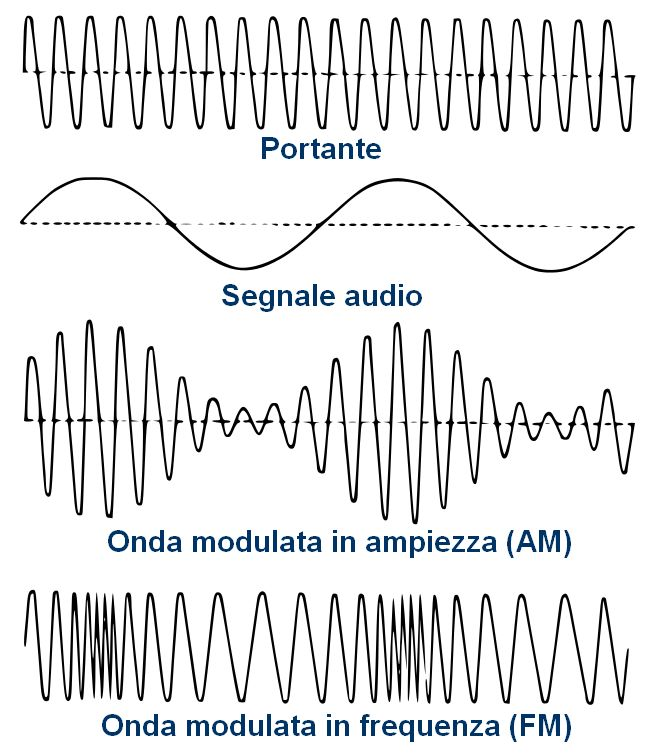
\includegraphics[scale=0.3]{amfm}
  \begin{figure}[h]
  	\centering
  	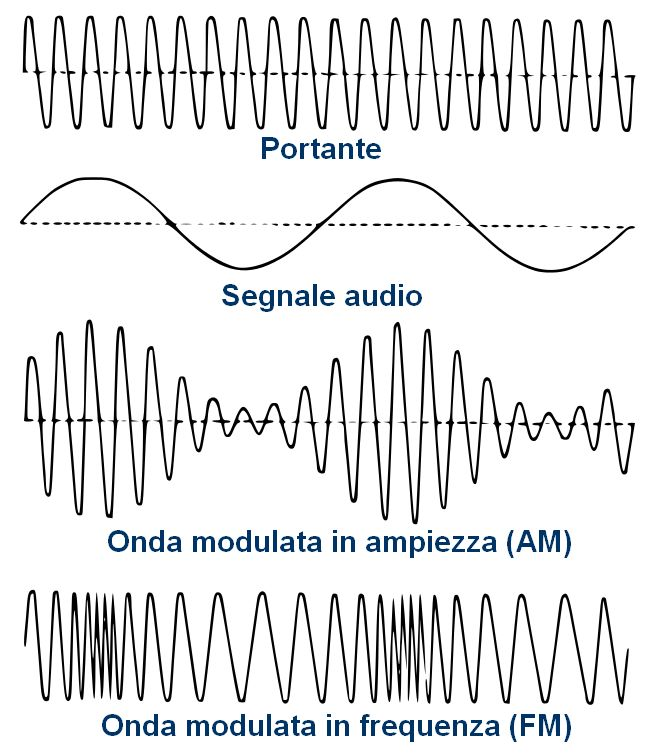
\includegraphics[scale=0.3]{amfm}
  	\caption{rappresentazione segnale modulato am e fm nel tempo}\label{fig:1}
  \end{figure}


\section{Modulazioni Digitali}
\label{sec:context}
\begin{itemize}
	\subsection{FSK}
  \item \textbf{FSK (frequency shifting key): } questa tecnica di modulazione codifica l' informazione variando la frequenza della portante in valori predefiniti, ad esempio per ottenere una codifica binaria alterna due frequenze diverse. Questa tecnica ha il vantaggio di essere facile nell'implementazione e poco soggetta ad interferenze tuttavia necessita di una maggiore larghezza di banda rispetto ad altre modulazioni digitali quali psk o ask.
  \cite{fsk}
  \subsection{ASK}
  \item \textbf{ASK (Amplitude shift keying): } la modulazione viene effettuata variando l' ampiezza del segnale portante alzandola o abbassandola in relazione alle informazioni da trasmettere, richiede un canale più affidabile in grado di ricevere anche i livelli di ampiezza più bassi. Trova ancora utilizzo nelle fibre ottiche e viene tuttora utilizzata la sua versione a codifica binaria (solo due livelli di potenza della portante presente/non presente) che prende il nome di OOF(on/off keying) in passato utilizzata anche per trasmettere messaggi in codice morse.
  \cite{ask}
  \subsection{PSK}
  \item \textbf{PSK (Phase Shift Keying): } questo tipo di modulazione codifica le informazioni in ingresso variando la fase della portante, ne esistono varie versioni che differiscono per il numero di valori diversi. La versione più semplice è la binaryPSK che varia di metà periodo mentre versioni come la 4PSK di un quarto e così via per la variante 8PSK e 16PSK. Tali possibili sfasature della portante vengono dette costellazione e vengono di norma rappresentate come coordinate complesse su un grafico. Sulle ascisse si trova la portante mentre sulle ordinate si trova in quadratura ovvero sfasata di 90°.La lunghezza del vettore fra l'origine e uno dei punti della costellazione rappresenta l' ampiezza del segnale modulato mentre l'angolo rappresenta la sfasatura rispetto alla portante. Esiste una variante di 4PSK detta QPSK che differisce per una disposizione della costellazione ruotata di 45°.
  \begin{figure}[h]
  	\centering
  	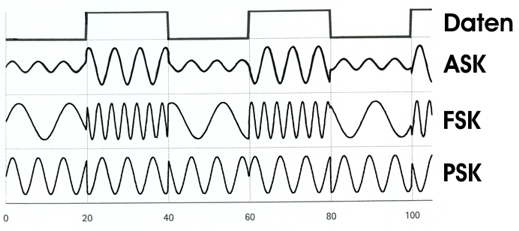
\includegraphics[scale=1.5]{digital}
  	\caption{rappresentazione segnale modulato nel tempo ASK FSK e PSK \cite{digit}}\label{fig:1}
  \end{figure}
	\subsection{QAM}
  \item \textbf{QAM (Quadrature amplitude modulation): } è una tecnica di modulazione simile a psk ma introduce la modulazione anche in ampiezza. La costellazione risulta avere punti non più equidistanti dall' origine. QAM come PSK presenta varianti che differiscono per il numero di punti sulla costellazione, in sistemi moderni si utilizzano anche 256 punti. QAM viene anche utilizzato per trasferire più flussi analogici contemporaneamente, questo particolare utilizzo fa si che QAM venga considerato anche come una tecnica di modulazione analogica. 
  \cite{qam}
  
  \begin{figure}[h]
	\centering
	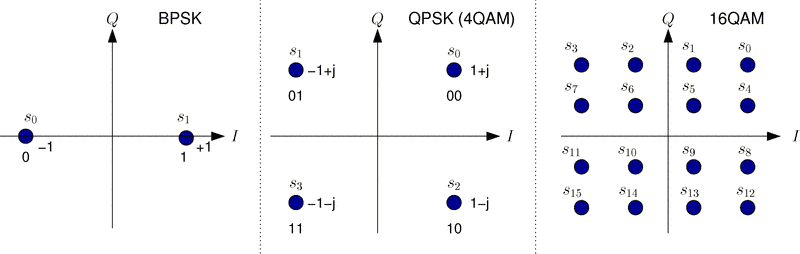
\includegraphics[scale=1.5]{constellation}
	\caption{Costellazioni BPSK, QPSK(4QAM), 16PSK \cite{psk-constellation}}\label{fig:1}
  \end{figure} 
  \end{itemize}
  %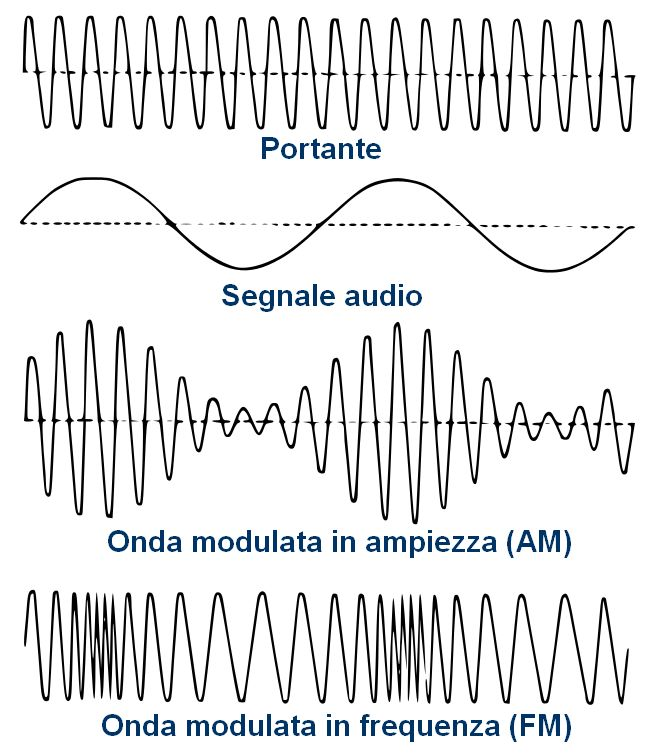
\includegraphics[scale=0.3]{amfm}


\section{OFDM}
\label{sec:problem}

Lorem ipsum dolor sit amet, consectetur adipiscing elit. Donec sed nunc orci. Aliquam nec nisl vitae sapien pulvinar dictum quis non urna. Suspendisse at dui a erat aliquam vestibulum. Quisque ultrices pellentesque pellentesque. Pellentesque egestas quam sed blandit tempus. Sed congue nec risus posuere euismod. Maecenas ut lacus id mauris sagittis egestas a eu dui. Class aptent taciti sociosqu ad litora torquent per conubia nostra, per inceptos himenaeos. Pellentesque at ultrices tellus. Ut eu purus eget sem iaculis ultricies sed non lorem. Curabitur gravida dui eget ex vestibulum venenatis. Phasellus gravida tellus velit, non eleifend justo lobortis eget.


